% \documentclass[sigconf]{acmart}
% 
% \usepackage{booktabs} % For formal tables
% \usepackage{color}
% \usepackage{textcomp}
% \usepackage{booktabs}
% \usepackage{graphicx}
% \usepackage{todonotes}
% \usepackage{multirow}
% \usepackage{subcaption}
% \usepackage{adjustbox}
% \usepackage[linesnumbered,ruled,vlined]{algorithm2e}
% \newcommand\mycheck[1]{\textcolor{red}{#1}}
% \newcommand\mycheckng[1]{\textcolor{red}{NG: #1}}
% \newenvironment{function1}[1][htb]
%   {\renewcommand{\thealgocf}{1}
%   \renewcommand{\algorithmcfname}{Function}% Update algorithm name
%    \begin{algorithm}
%   }{\end{algorithm}}  
% 
% 
% \frenchspacing
% \setlength{\pdfpagewidth}{8.5in}
% \setlength{\pdfpageheight}{11in}
% % \pdfinfo{
% % /Title (Insert Your Title Here)
% % /Author (Put All Your Authors Here, Separated by Commas)}
% %\setcounter{secnumdepth}{0}  
%  \begin{document}
% % The file aaai.sty is the style file for AAAI Press 
% % proceedings, working notes, and technical reports.
% %
% \title{On the effectiveness of multiple reviewers in a peer-review system: A case study of two high impact Physics journals}
% %\subtitle{A large-scale comparison of single vs multiple peer-review system}
% % \author{AAAI Press\\
% % Association for the Advancement of Artificial Intelligence\\
% % 2275 East Bayshore Road, Suite 160\\
% % Palo Alto, California 94303\\
% % }
% \renewcommand{\shorttitle}{Effectiveness of multiple reviewers in a peer-review system}
% 
% \begin{abstract}
% Peer-review is considered as one of the most  important steps to maintain the quality of research publication.
% The research community is however reaching a consensus that although scientific peer-review is highly relevant, 
% it is nonetheless flawed. One of the most important steps in the peer-review process is the assignment of peers or referees who are 
% handed the responsibility of judging the quality of the submission. Hence the training and the knowledge of all the referees are critical in proper quality judgment of the work. It is usually believed that to make the review process as fair as possible, decisions 
% from multiple referees should be favored over a single referee.  
% We in this paper consider peer-review data 
% of leading scientific journals and systematically study the cases where a single reviewer is involved and compare these with the cases where multiple reviewers are 
% involved. We observe that on average single refereed papers are more cited compared to multi-refereed papers. However, papers reviewed by multiple referees constitute the majority of the most cited (top 25\%) papers in our dataset. Further, analyzing the review reports we find that in a multi-referee system, in many cases the referees fail to reach consensus on their decision possibly leading to wrong overall judgments. All these observations lead us to believe 
% that a multiple referees in the context of a peer-review system, although effective, suffers due to assignment of irreconcilable referees. This observation leads us to further propose a 
% framework based on genetic algorithms to recommend compatible referee groups (based on the time since last assignment and fraction of papers 
% accepted) in case of a multiple referee system. 
% In fact across the two datasets our framework on average could correctly recommend 
% reviewer groups in $\sim$ 78\% of the cases showing that multi-referee groups can work well only when the group members are chosen appropriately. Our framework further ensures fairness in referee assignment by not encumbering the better-performing referees. 
%  
% \end{abstract}
% 
% \begin{CCSXML}
% <ccs2012>
% <concept>
% <concept_id>10003120.10003130.10003233</concept_id>
% <concept_desc>Human-centered computing~Collaborative and social computing systems and tools</concept_desc>
% <concept_significance>500</concept_significance>
% </concept>
% </ccs2012>
% \end{CCSXML}
% 
% \ccsdesc[500]{Human-centered computing~Collaborative and social computing systems and tools}
% 
% 
% % We no longer use \terms command
% %\terms{Theory}
% 
% \keywords{peer-review; genetic algorithm; citation; reviewer}
% 
% 
% \maketitle

%\vspace{-8mm}
% \noindent
%\section{Introduction}
The scientific community relies heavily on the peer-review system to judge the quality of a new research contribution. In this process a set of 
peers or reviewers are handed the responsibility of judging whether the work is flawed and should be discarded or is relevant enough to be brought to the 
notice of the research community. Since the reviewers are the most important entities of the entire peer-review process, their knowledge and training are 
highly critical to the proper functioning of the review process. 
In fact in may cases when more than one referees are involved in reviewing a paper, lack of consensus among them might make it difficult for the editor to judge the 
true quality of the work, which then might lead to a severe mistake.

\noindent{{\bf Single or multiple reviewers:}}
So a natural query arises: whether peer-reviewing comprising multiple referees should be preferred over a single referee system? 
To answer this question, we in this paper for the first time, 
analyze the peer-review information of all the papers that were submitted to two leading physics journals together consisting of approximately $36k$ papers with 
about $19m$ lines of review texts. 
An exploratory analysis of citation information of the papers reveals that papers 
reviewed by multiple referees, on acceptance tend to be cited less (on average) while on rejection tend to be cited more (on average) compared to the papers which get reviewed 
by a single referee.
However, papers reviewed by multiple reviewers constitute the majority of the most cited (top 25\%) papers. 
In fact, the observations 
are consistent across both these datasets. The dichotomy in this observations raises a natural question 
that why multiple refereeing does not work well on average. We hypothesize that this is mainly due to lack of consensus among the referees in the multi-reviewer system.

\noindent{{\bf Lack of consensus among reviewers:}}
In~\cite{cole1981chance} the authors demonstrated that in multi-refereed papers the referees often fail to reach consensus. As an immediate next step following the 
previous observations, we investigate the review reports of the multi-refereed papers. Leveraging several natural language processing (NLP) tools we 
establish the lack of consensus among reviewers for such papers. In fact, we observe that in terms of report length, sentiment and content, the referees 
differ in almost 30\% of the cases on average across the two datasets.

\noindent{{\bf Analyzing multi-referee behavior:}} 
Further analysis of the peer-review system reveals that 
the performance of a reviewer can be quantified by his/her  
 (a). frequency of assignment and (b). tendency to be too critical (tends to reject most of the papers assigned to them) 
or too liberal (tends to accept majority of assignments). The discordance also occurs when such reviewers are grouped together, which perhaps
leads to acceptance of paper without due diligence. In contrast, we find that even when under-performing
reviewers are grouped with well-performing reviewers, the overall quality of acceptance improves. 
Remarkably, we also observe, that the most under-performing groups have the highest lack of consensus, which further corroborates our hypothesis.

\if{0}
In~\cite{sikdar2016anomalies} the authors pointed out several factors which might be indicative of anomalous behavior (under-performance) of 
the editors and the referees. We observe 
that the anomalous editors often tend to assign multiple referees. All the above results should indicate that it is better to assign single referees instead 
of multiple ones. But a deeper analysis indicates that anomalous referees when assigned a paper as single reviewer often fail to correctly judge the 
quality of the paper while when part of a multi-referee system performs much better. We further observe that while for some topics generally single reviewer 
is assigned for the paper, for others multiple reviewers are assigned. This might be due to the fact that some topics are so definitive that it is difficult 
to find multiple knowledgeable reviewers while for the generic topics it is easier to find multiple reviewers.
\fi


\noindent{{\bf Recommending reviewer groups:}}
From the above observations we hypothesize that multi-referee systems mostly fail due to lack of proper selection and the assignment of the referees. 
We in this paper propose a systematic scheme 
for recommending reviewer groups to the editor. We argue that the problem of assigning multiple referees to a paper is similar to the problem of forming compatible 
groups from a population, which has already been studied in great detail in the context of collaborative learning. In fact, genetic algorithm (GA) 
based frameworks have been shown to be very effective in such a setting \cite{moreno2012genetic,ani2010method}. 
We hence propose a GA based framework which, given a paper, 
its topic and a reviewer pool with past information, is able to recommend a 
set of groups of compatible referees to assist the editor in assignment of referees. 
We observe that in cases where the reviews led to acceptance and the paper garnered a 
large number of citations, our algorithm is able to correctly identify almost \textbf{ $78\%$} of the group of referees 
involved on average across the two datasets. 
\if{0}
In the lines of~\cite{sikdar2016anomalies}, we further observe that the accept ratio of a 
reviewer (fraction of papers accepted) and the time to the last assignment are indicators of reviewer performance which we leverage to calculate 
the fitness score of each reviewer and a reviewer group as well.  
\fi

\noindent{{\bf Importance of editor intervention:}}
The above results might give a false impression that given a set of topics and reviewer history, 
our system can recommend reviewer groups without the expert intervention of the editor. 
Using a carefully designed simulation setup, we show that intervention of the editor in selecting a reviewer group 
from the set of recommended groups is highly critical to the proper functioning of the system in long term. In fact 
we show that the ability of correctly identifying the reviewer groups reduces to almost  \textbf{ $45\%$ (from $78\%$)} if 
the editor is not involved in the peer-review process.


\medskip


%\vspace{-4mm}
%\noindent
\section{Related work}
\label{related_works}
The effectiveness of peer-review system has often been debated. Researchers have pointed out its several limitations~\cite{ingelfinger1974peer,relman1989good,smith2006peer}. 
In fact, authors in~\cite{cole1981chance} showed that 
reviewers often fail to reach consensus when judging the quality of the contribution while~\cite{braatz2014papers} points out that 
rejected papers are often cited more in the long run. Nevertheless, little work has been done toward systematic analysis and improvement of the 
system~\cite{graffy2006improving}. That blinding can improve the quality of the reviews, has been demonstrated in~\cite{mcnutt1990effects}.~\cite{caswellimproving} pointed 
out that incentives for reviewers could encourage them doing a better job. In~\cite{sikdar2016anomalies} the authors 
point out several indicators for anomalous behavior of the referees and the editors. In fact, they were able to filter out 
anomalous editors and reviewers leveraging anomaly detection algorithms. 

On the other hand, there have been a lot of work on the formation of teams of experts whose goal is to complete a given 
project~\cite{anagnostopoulos2010power,anagnostopoulos2012online, lappas2009finding,agrawal2014grouping,pragarauskas2012multi}. A trend in this line of work is to formulate
the team formation problem as an integer linear program
(ILP), and then focus on finding an optimal match
between people and the demanded functional requirements.
Widely used techniques in solving these problems include simulated
annealing~\cite{baykasoglu2007project}, branch-and-cut~\cite{zzkarian1999forming} or genetic algorithms~\cite{ani2010method}.~\cite{agrawal2014grouping} proposed 
a way of creating study groups in an educational setting so that the overall gain for the 
students is maximized. Another set of works leverage the underlying social network among the individuals as a proxy for compatibility and propose 
techniques for creating groups so as to match the requirements 
of a co-operative task~\cite{majumder2012capacitated,mcdonald2003recommending,wolf2009mining,li2010team}. 
In this paper we consider the review information of two leading scientific 
journals (JHEP -- Journal of High Energy Physics and JSTAT -- Journal of Statistical Mechanics: Theory and Experiment) and propose a scheme 
for allocating referees for a submitted paper. Anonymity of the reviewers and absence of any kind of underlying network 
prevents us from using any of the existing network based approaches. Formulating it as an ILP also appears difficult due to unavailability of any obvious optimization function.
To the best of our knowledge this is the first work which formulates the referee recommendation in peer-review system as a group formation problem 
leveraging genetic algorithms. We believe our findings could be useful in increasing the effectiveness of the peer-review system.

\begin{table}[]
\centering
\caption{Some general information related to the two datasets.}
\label{tab:data}
\scalebox{0.85}{
\begin{tabular}{l|l|l}
\hline
                                                                                      & JHEP  & JSTAT \\ \hline\hline
\# papers                                                                             & 28871 & 6106  \\ \hline
\# accepted papers                                                                    & 20384 & 3528  \\ \hline
\begin{tabular}[c]{@{}l@{}}Fraction of multi-reviewed \\ papers\end{tabular}           & 0.12  & 0.43  \\ \hline
\begin{tabular}[c]{@{}l@{}}\# Editors with at least one \\ assignment\end{tabular}    & 95    & 148   \\ \hline
\begin{tabular}[c]{@{}l@{}}\# Reviewers with at least \\ one assignment\end{tabular}  & 3976  & 2647     \\ \hline
\begin{tabular}[c]{@{}l@{}}Average number of \\ reviewers per paper\end{tabular}      &  1.03     & 1.42      \\ \hline
\begin{tabular}[c]{@{}l@{}}Average number of \\ authors per paper\end{tabular}        &  2.87     & 2.32      \\ \hline
\begin{tabular}[c]{@{}l@{}}Average number of \\ assignments per reviewer\end{tabular} &  6.48     &  2.56     \\ \hline
\# Unique keywords                                                                    & 201 & 562  \\ \hline
\end{tabular}}
\end{table}

\medskip

%\vspace{-3mm}
%\noindent
\section{Dataset}
\label{dataset}
We consider datasets of two physics journals (i) Journal of High Energy Physics (JHEP) and 
(ii) Journal of Statistical Mechanics: Theory and Experiment (JSTAT). JHEP is a leading physics 
journal with an impact factor of 6.023\footnote{http://iopscience.iop.org/journal/1126-6708} and 
publishes theoretical and experimental papers in high energy physics while JSTAT publishes papers in statistical physics and has 
an impact factor of 2.091\footnote{http://iopscience.iop.org/journal/1742-5468}. 
JSTAT is more interdisciplinary and attracts papers from a wide range of researchers from physicists to computer scientists while for JHEP the papers published are 
limited to only very specific topics. 
Note that these are two diverse datasets; while JHEP predominantly follows a single-referee format with only around 10\% papers being reviewed by multiple referees, 
JSTAT is more open to a multiple-referee format (close to 43\% papers are multi-refereed). 

\noindent{\bf JHEP} dataset contains information of 28871 papers which were submitted between 1997 and 2015. The meta information available for each paper includes 
(i) the title, (ii) the list of authors, (iii) the final decision (accept/reject/withdrawn), (iv) the keywords related to the paper, (v) the long term citation 
(cumulative citations received 
from date of publication to 2015), (v) the submission date, (vi) the publication date (in case the paper was accepted) and (vii) the abstract. 
Moreover, for each paper the whole review process information is available which includes (i) the assigned editor, (ii) the assigned reviewers, (iii) the report submitted 
by the reviewers in each round of review and (iv) the citation information of the accepted papers.
%We also obtain the citation information of the rejected papers by querying the inspire database\footnote{http://inspirehep.net/?ln=en}. 
%Some general information related to the JHEP dataset is noted in 
%table \ref{tab:data}.

\noindent{\bf JSTAT} dataset contains information of 6106 papers which were submitted between 2004 and 2016. The meta information available for each paper is same as that of the 
JHEP dataset. 
All the above information for both the datasets were made available to us by the respective publishing houses.

\noindent{\bf Information crawled:} For JHEP we further queried the $inspire$ database\footnote{http://inspirehep.net/?ln=en} to obtain citation and other meta information 
of the rejected papers.  
For JSTAT the citation information of the papers (both accepted and rejected) were not available. Hence, we collected the titles of all the papers and queried the ``scopus''\footnote{https://www.scopus.com/home.uri}
database to obtain the citation information of the papers (both accepted and rejected). 
Note that this is the long term citation i.e., the cumulative citations received from the date of publication to 2016. Throughout the paper any reference to citation 
would mean this cumulative citation unless otherwise specified.
%Since we have the titles for both the accepted and the rejected papers, we could crawl the citation information for both these classes. 
Some general information related to the two datasets is noted in table~\ref{tab:data}.
Further, for both JHEP and JSTAT, each paper is assigned a set of keywords (at least 2 and at most 4) by the publisher which represents the related topic of a paper. 

%\textcolor{blue}{Sandipan: It was there for JHEP but not for JSTAT. Rejected papers were tracked through the tile and author list.}
%table \ref{tab:data}.
% \begin{table}[]
% \centering
% \caption{Some general information related to the two datasets.}
% \label{tab:data}
% \begin{tabular}{l|l|l}
% \hline
%                                                                                       & JHEP  & JSTAT \\ \hline\hline
% \# papers                                                                             & 28871 & 6106  \\ \hline
% \# accepted papers                                                                    & 20384 & 3528  \\ \hline
% \begin{tabular}[c]{@{}l@{}}Fraction of multi-reviewed \\ papers\end{tabular}           & 0.12  & 0.43  \\ \hline
% \begin{tabular}[c]{@{}l@{}}\# Editors with at least one \\ assignment\end{tabular}    & 95    & 148   \\ \hline
% \begin{tabular}[c]{@{}l@{}}\# Reviewers with at least \\ one assignment\end{tabular}  & 3976  & 2647     \\ \hline
% \begin{tabular}[c]{@{}l@{}}Average number of \\ reviewers per paper\end{tabular}      &  1.03     & 1.42      \\ \hline
% \begin{tabular}[c]{@{}l@{}}Average number of \\ authors per paper\end{tabular}        &  2.87     & 2.32      \\ \hline
% \begin{tabular}[c]{@{}l@{}}Average number of \\ assignments per reviewer\end{tabular} &  6.48     &  2.56     \\ \hline
% \end{tabular}
% \end{table}

\begin{figure}
 \centering
 \includegraphics[scale = 0.26]{figures/citation_jhep_1.eps}
 \caption{\label{citation:jhep} Citation distribution of the multi-refereed and single-refereed papers for (Left) accepted and (Right) rejected papers for JHEP dataset.\vspace{-4mm}} 
\end{figure}

\begin{figure}
 \centering
 \includegraphics[scale = 0.26]{figures/citation_jstat_1.eps}
 \caption{\label{citation:jstat} Citation distribution of the multi-refereed and single-refereed papers for (Left) accepted and (Right) rejected papers for JSTAT dataset.\vspace{-2mm}}
\end{figure}

\begin{figure}
 \centering
 \includegraphics[scale = 0.26]{figures/best_paper.eps}
 \caption{\label{fig:best} Fraction of multi-refereed papers in the top $k$ most cited papers where $k = 1,50,100,500,1000,2000$.\vspace{-4mm}}
\end{figure}

\begin{figure*}[!ht]
 \centering
 \begin{subfigure}[b]{0.49\textwidth}
 \centering
  \includegraphics[scale = 0.28]{figures/jhep_all.eps}
  \caption{\label{disagree:jhep}JHEP}
 \end{subfigure}%
 ~
 \begin{subfigure}[b]{0.49\textwidth}
 \centering
  \includegraphics[scale = 0.28]{figures/jstat_all.eps}
  \caption{\label{disagree:jstat}JSTAT}
 \end{subfigure}

 \caption{ Fraction of cases where the reviewers disagreed with respect to (1) length (2) sentiment and (3) content for (a) JHEP and (b) JSTAT 
  datasets.\vspace{-4mm}}
  
\end{figure*}


\medskip

%\vspace{-3mm}

% \begin{figure}
%  \centering
%  \includegraphics[scale = 0.4]{./texfiles/Chapter_4/cikm_17/figures/citation_jhep_1.eps}
%  \caption{\label{citation:jhep} Citation distribution of the multi-refereed and single-refereed papers for (Left) accepted and (Right) rejected papers for JHEP dataset.} 
% \end{figure}
% 
% \begin{figure}
%  \centering
%  \includegraphics[scale = 0.4]{./texfiles/Chapter_4/cikm_17/figures/citation_jstat_1.eps}
%  \caption{\label{citation:jstat} Citation distribution of the multi-refereed and single-refereed papers for (Left) accepted and (Right) rejected papers for JSTAT dataset.}
% \end{figure}
% 
% \begin{figure}
%  \centering
%  \includegraphics[scale = 0.28]{./texfiles/Chapter_4/cikm_17/figures/best_paper.eps}
%  \caption{\label{fig:best} Fraction of multi-refereed papers in the top $k$ most cited papers where $k = 1,50,100,500,1000,2000$.}
% \end{figure}


% \begin{figure*}
% \centering
% \begin{tabular}{cc}
% \includegraphics[scale = 0.28]{./texfiles/Chapter_4/cikm_17/figures/jhep_all.eps} & \includegraphics[scale = 0.28]{./texfiles/Chapter_4/cikm_17/figures/jstat_all.eps}
% \end{tabular}
% \caption{\label{disagree:jhep} Fraction of cases where the reviewers disagreed with respect to (1) length (2) sentiment and (3) content for (a) JHEP and (b) JSTAT 
%   datasets.}
% \end{figure*}  

\noindent
\section{Single vs multiple referee system}
\label{mvs}
%\mycheck{Put in significance test results....}
In this section we systematically compare the papers which are reviewed by multiple peers (which we call multi-refereed) with those which are reviewed by a single peer 
(which we call single-refereed). 
To this aim 
we first compare the long term citations of both of these classes of papers. We further analyze the review reports received from the peers and check whether 
the reviewers disagreed in their opinion about the paper. 

\begin{figure}
 \centering
 \includegraphics[scale = 0.35]{./texfiles/Chapter_4/cikm_17/figures/citation_jhep_1.eps}
 \caption{\label{citation:jhep} Citation distribution of the multi-refereed and single-refereed papers for (Left) accepted and (Right) rejected papers for JHEP dataset.} 
 \vspace{3mm}
 \end{figure}

\begin{figure}
 \centering
 \includegraphics[scale = 0.35]{./texfiles/Chapter_4/cikm_17/figures/citation_jstat_1.eps}
 \caption{\label{citation:jstat} Citation distribution of the multi-refereed and single-refereed papers for (Left) accepted and (Right) rejected papers for JSTAT dataset.}
 \vspace{3mm}
 \end{figure}



\subsection{Citation}

We first look into the long term citations of the papers which are reviewed by multiple peers as well as those reviewed by a single peer. 
We consider the accepted papers and the rejected papers separately. 
In figure~\ref{citation:jhep}(a) we plot the cumulative distribution of the citations received by the accepted papers belonging to the single and the multi-refereed classes 
for JHEP. 
We observe that the accepted papers which are multi-refereed tend to garner less citations (mean 30.62) in the long run as compared to the single-refereed 
(mean 36.48) ones $(p < 0.01)$. 
An exact opposite trend is observed in case of the rejected papers (mean = 12.8 (multi), 8.42 (single),  $p< 0.02$) (refer to figure~\ref{citation:jhep}(b)). 
%Note that for JHEP, majority of 
%the papers are single-refereed and only $10\%$ of the 
%papers are multi-refereed. So to make the comparison fair we did not consider the whole population of single-refereed paper; rather we randomly sampled 
%out an equal number of single-refereed papers. Strikingly, we find that the results are similar across all the $5$ different samples we test. Statistical significance 
%test further 

We repeat the same experiment for the JSTAT papers as well. The corresponding plots for the accepted and the rejected papers are shown in 
figures~\ref{citation:jstat}(a) and~\ref{citation:jstat}(b) respectively. Although for accepted papers the mean citation ($26.82$) for the single referee 
case is marginally larger than the 
multi-referee case (mean citation $= 24.26$), for rejected papers,    
%We observe a similar behavior here as well. 
mean citations for multi-refereed (10.92) and single-refereed (6.86) papers are significantly $(p < 0.02)$ different.
These results together 
indicate that when working in groups the reviewers often fail (on average) to correctly judge the quality of the paper.

\begin{figure}
 \centering
 \includegraphics[scale = 0.25]{./texfiles/Chapter_4/cikm_17/figures/best_paper.eps}
 \caption{\label{fig:best} Fraction of multi-refereed papers in the top $k$ most cited papers where $k = 1,50,100,500,1000,2000$.}
 \vspace{4mm}
\end{figure}

\begin{figure*}
\centering
\begin{tabular}{cc}
\includegraphics[scale = 0.26]{./texfiles/Chapter_4/cikm_17/figures/jhep_all.eps} & \includegraphics[scale = 0.26]{./texfiles/Chapter_4/cikm_17/figures/jstat_all.eps}
\end{tabular}
\caption{\label{disagree:jhep} Fraction of cases where the reviewers disagreed with respect to (1) length (2) sentiment and (3) content for (a) JHEP and (b) JSTAT 
  datasets.}
  \vspace{4mm}
\end{figure*}  

\subsection{Top cited papers}

The above results would indicate that it is always better to assign a single reviewer instead of multiple reviewers. However, 
a deeper and a more microscopic analysis portrays a very different picture. 
On  computing the proportion of multi-refereed papers in the top $k$ most cited papers (where $k = 1,50,100,500,1000,2000$) we observe that the 
fraction is very high for really top cited papers and then it decreases (refer to figure~\ref{fig:best}).
In fact, the most cited paper in our dataset is also multi-refereed.  
This indicates that sincere, knowledgeable multi-review indeed helps in identifying impactful papers. 
%which drops as we increase $k$ which indicates the least cited papers are mostly the single-reviewed ones.}
%On considering 100 most cited papers in the JSTAT dataset we observed that 45 of them are multi-reviewed ones while 
We also observe that for 100 least cited papers only 26 of them are 
multi-reviewed which again indicates single-review may lead to several unappealing entry. 
%This indicates that on average single-reviewed papers might be getting more citation but they also constitute the majority of least cited ones.  \mycheckng{Cant we draw a graph checking top 10/top 100 etc. and this should be put just before conflict}

\subsection{Conflict in review reports}
There may be various reasons behind the average under-performance of multiple reviewer system, 
one of which could be the difference in opinions among the reviewers whereby the paper may have got accepted despite 
a subset of  reviewers  not recommending the paper.
%An immediate next step would be to check whether the reviewers, when working in groups agree on their opinion about the quality of the paper.  For this analysis we specifically consider the multi-refereed papers. 
Understanding this aspect from the dataset is difficult as 
%Note that in case of multi-refereed papers 
although the review reports from the respective peers are accessible, their final decisions (accept/reject/major-review) are 
not explicitly available making it difficult to understand the differences in opinions. 
Therefore we leverage on traditional natural language processing tools 
to segregate papers according to reviewers' agreement/disagreement and then check their impact. Accepted and rejected papers are considered separately.
We specifically look into three factors - (i) length (ii) sentiment and (iii) content of the review report of all the involved referees. Note that 
in this work we do not aim to identify the most distinguishing features for identifying or 
quantifying differences in opinion from the review reports. The proposed features albeit crude, are sufficiently adequate to unfurl the 
dissonance among the referees which is our 
prime intention.
%{We perform the experiments separately for the accepted and the rejected papers.}
%to check whether the peers agree.  \mycheckng{are we working only on accepted papers - mention that explicitly}


\subsubsection{Length}

We start by comparing the length of the review reports sent by each peer assigned for a given paper. Our hypothesis is that if the peers have a similar 
opinion on the assigned paper, the length of their reports would be typically close. To this aim, we calculate the standard deviation of the lengths 
(i.e., number of words) of the reviewer reports for every round of review for each paper and use it as a metric to judge whether a particular round is discordant 
(i.e., the reviewers disagreed) or concordant (i.e., the reviewers agreed). If the standard deviation is greater than the length of the smallest-length review, 
we classify the review round as discordant. Otherwise, we classify the review round as concordant.
In figure~\ref{disagree:jhep}(1) we plot the fraction of multi-refereed papers where the peers disagreed in case of JHEP. The corresponding result for 
JSTAT is shown in figure~\ref{disagree:jstat}(1). We observe that for JHEP the peers disagree in almost $35\%$ of the cases in the first round of the review 
for the papers which are finally accepted and close to $30\%$ for the papers which are rejected. The corresponding numbers for JSTAT are $30.5\%$ and $35.7\%$ 
respectively. In fact, even in the second round of reviews the peers tend to disagree as well (refer to figure~\ref{disagree:jhep}(1) and~\ref{disagree:jstat}(1)).

\subsubsection{Sentiment}

We next analyze the sentiments latent in the review reports. If for a document all the reviewers are of positive opinion or of negative opinion we 
consider it as a concordant case. If the opinion of at least one of the reviewers differ from the rest we consider it as discordant. 
To calculate the sentiment score of the reports we use nltk-sentiwordnet toolkit\footnote{http://www.nltk.org/}. In figures~\ref{disagree:jhep}(2) and~\ref{disagree:jstat}(2) 
we plot the fraction of discordant cases for both the accepted and rejected papers for JHEP and JSTAT respectively. We observe that for JHEP, across the two versions on average 
the referees 
disagree in around 20\% of the cases for the accepted papers and in around 30\% of the cases for the rejected papers. In case of JSTAT the disagreement is even higher 
with the corresponding numbers being around 40\% and 35\% respectively. 


\subsubsection{Content}

%In multi-refereed cases although we have the content of the report, the explicit score of the reviewer is missing. 
To further analyze if the contents in the review reports 
from multiple referees are conflicting, we perform a term frequency-inverse document frequency (TF-IDF) based analysis to estimate the extent of difference in the referee 
opinions. For this purpose, we first need to construct a vocabulary representing the typical review report for an accepted (rejected) paper. Toward this objective, we collate the 
final round report of all the single-refereed accepted (rejected) papers. These are the texts where 
we are sure whether the review led to an acceptance (a rejection) of the paper. Next we construct the respective TF-IDF vectors corresponding to the accepted (rejected) 
papers from the collated text. Let us call these {\em acceptance} ({\em rejection}) vectors. Finally, we compare the TF-IDF vector corresponding to each report of the 
multi-refereed papers to check if it aligns more with
the acceptance vector or the rejection vector. If the reviews from all the referees align to the same vector we consider it as a concordant case. Otherwise we consider 
it as a discordant case. 
In figures~\ref{disagree:jhep}(3) and~\ref{disagree:jstat}(3) we plot the fraction of discordant cases for JHEP and JSTAT respectively. We observe that for JHEP, 
across the two versions/rounds the reviewers disagree on average in almost 30\% of the cases for accepted papers and close to 25\% on average for rejected papers. 
For JSTAT the reviewers disagree on 24\% cases in version 1 and 26\% cases in version 2 for accepted papers. The corresponding numbers for 
the rejected papers are 17\% and 27\% respectively.

% \begin{figure*}[!ht]
%  \centering
%  \includegraphics*[scale = 0.35]{figures/jstat_all.eps}
%  \caption{\label{disagree:jstat} Fraction of cases where the reviewers disagreed with respect to (a) length (b) sentiment and (c) content for JSTAT dataset}
% \end{figure*}
% \begin{figure*}[!ht]
%  \centering
%  \includegraphics*[scale = 0.35]{figures/jhep_all.eps}
%  \caption{\label{disagree:jhep} Fraction of cases where the reviewers disagreed with respect to (a) length (b) sentiment and (c) content for JHEP dataset. For each figure results for review round 1 and 2 are reported.  \mycheckng{Make JHEP and JSTAT figure together} }
% \end{figure*}
% 
% \begin{figure*}[!ht]
%  \centering
%  \includegraphics*[scale = 0.35]{figures/jstat_all.eps}
%  \caption{\label{disagree:jstat} Fraction of cases where the reviewers disagreed with respect to (a) length (b) sentiment and (c) content for JSTAT dataset}
% \end{figure*}



In table~\ref{tab:jacc} we present the Jaccard similarity between the discordant cases as detected by the above three metrics (length, sentiment and content) to check 
whether the same cases are identified by all the three metrics. 
We observe high Jaccard similarity between cases identified as discordant by length and sentiment. This similarity is a bit lower with the cases identified as discordant 
by content analysis.

\begin{table}[]
\centering
\caption{Jaccard similarity between the cases identified as discordant by the different metrics.}
\label{tab:jacc}
\begin{tabular}{c|c|c|c}
\hline
          & Length & Sentiment & Content \\ \hline
Length    &    1.0    &   0.63        &  0.37       \\ 
Sentiment &    0.63    &   1.0        &  0.29       \\ 
Content   &    0.37    &   0.29        &  1.0       \\ \hline
\end{tabular}
\end{table}



\begin{figure}
 \centering
 \includegraphics[scale = 0.3]{./texfiles/Chapter_4/cikm_17/figures/citation_mul_all.eps}
 \caption{\label{con:citation} Cumulative distribution function of citations for single refereed papers and concordant multi-refereed papers 
 in terms of (a) length, (b) sentiment 
 and (c) content for JHEP. %We randomly selected single-reviewed papers equal in number to the concordant multi-reviewed sets for each type.
 }
\end{figure}
% \subsection{Deeper analysis of multi-reviewed papers}
% \textcolor{blue}{The above results would indicate that it is always better to assign single reviewer instead of multiple reviewers. But a deeper analysis reveals a different 
% aspect. On considering 100 most cited papers in the JSTAT dataset we observed that 45 of them are multi-reviewed ones while for 100 least cited papers only 26 of them are 
% multi-reviewed. In fact the highest cited paper (with 1838 citations) is multi-reviewed. 
% This indicates that on average single-reviewed papers might be getting more citation but they also constitute the majority of least cited ones.
% We further plot the proportion of multi-reviewed papers in top $k$ most cited papers where $k = 1,50,100,500,1000,2000$ in figure \ref{fig:best}. We observe that the 
% fraction drops as we increase $k$ which indicates the least cited papers are mostly the single-reviewed ones.}

%\textcolor{blue}{We previously showed that for multi-reviewed papers, often the reviewers reach consensus. If we consider the concordant (where the reviewers agreed) and discordant (where the reviewrs
\subsection{Impact of discordance}
If we consider the concordant (where the reviewers agreed) and discordant (where the reviewers
disagreed) papers separately, we observe that the concordant papers are often highly cited in the long run. In figure~\ref{con:citation} 
we plot the cumulative distribution function 
of citations received by the concordant papers and that received by the single-refereed ones for the JHEP dataset. 
%\mycheck{Put in the mean values as well as the p-value}.
In all the three cases (length, sentiment and content), average citation (32.65, 35.45, 31.67 respectively) of concordant multi-refereed 
accepted papers tend to be more compared to that of the single-refereed ones (30.39). We 
observe an exact opposite behavior in case of the discordant papers (refer to figure~\ref{con:citation_dis}). 
More specifically average citation of length discordant papers (22.33) differ significantly ($p < 0.03$) from average citation of single refereed ones. Similar trend is observed 
for sentiment discordant (mean $=19.23$, $p < 0.02$) and content discordant (mean $=21.36$, $p < 0.03$) cases. 
This goes to show that if the reviewers are chosen correctly, the multi-referee setup can perform better than a single-referee setup. 

As we shall see in the next section, the impact  of  the papers can be understood in further details if we  investigate the performance of the reviewers assigned to review 
the papers. 
%check the patterns of assingment of editors who are responsible for accepting under-performing papers which we do next.}

%To summarize we observe that papers reviewed and accepted by multiple peers on average fail to generate large number of citations as compared to the 
%single-refereed ones. We further leverage NLP tools and conclude that the reviewers often disagree on their opinion of the paper which in many cases possibly lead to incorrect judgment. 

% \begin{figure}
%  \centering
%  \includegraphics[scale = 0.3]{figures/citation_mul_all.eps}
%  \caption{\label{con:citation} Cumulative distribution function of citation for single reviewed papers and concordant multi-reviewed papers in terms of (a) length, (b) sentiment 
%  and (c) content. We randomly selected single-reviewed papers equal in number to the concordant multi-reviewed sets for each type.}
% \end{figure}

\begin{figure}
 \centering
 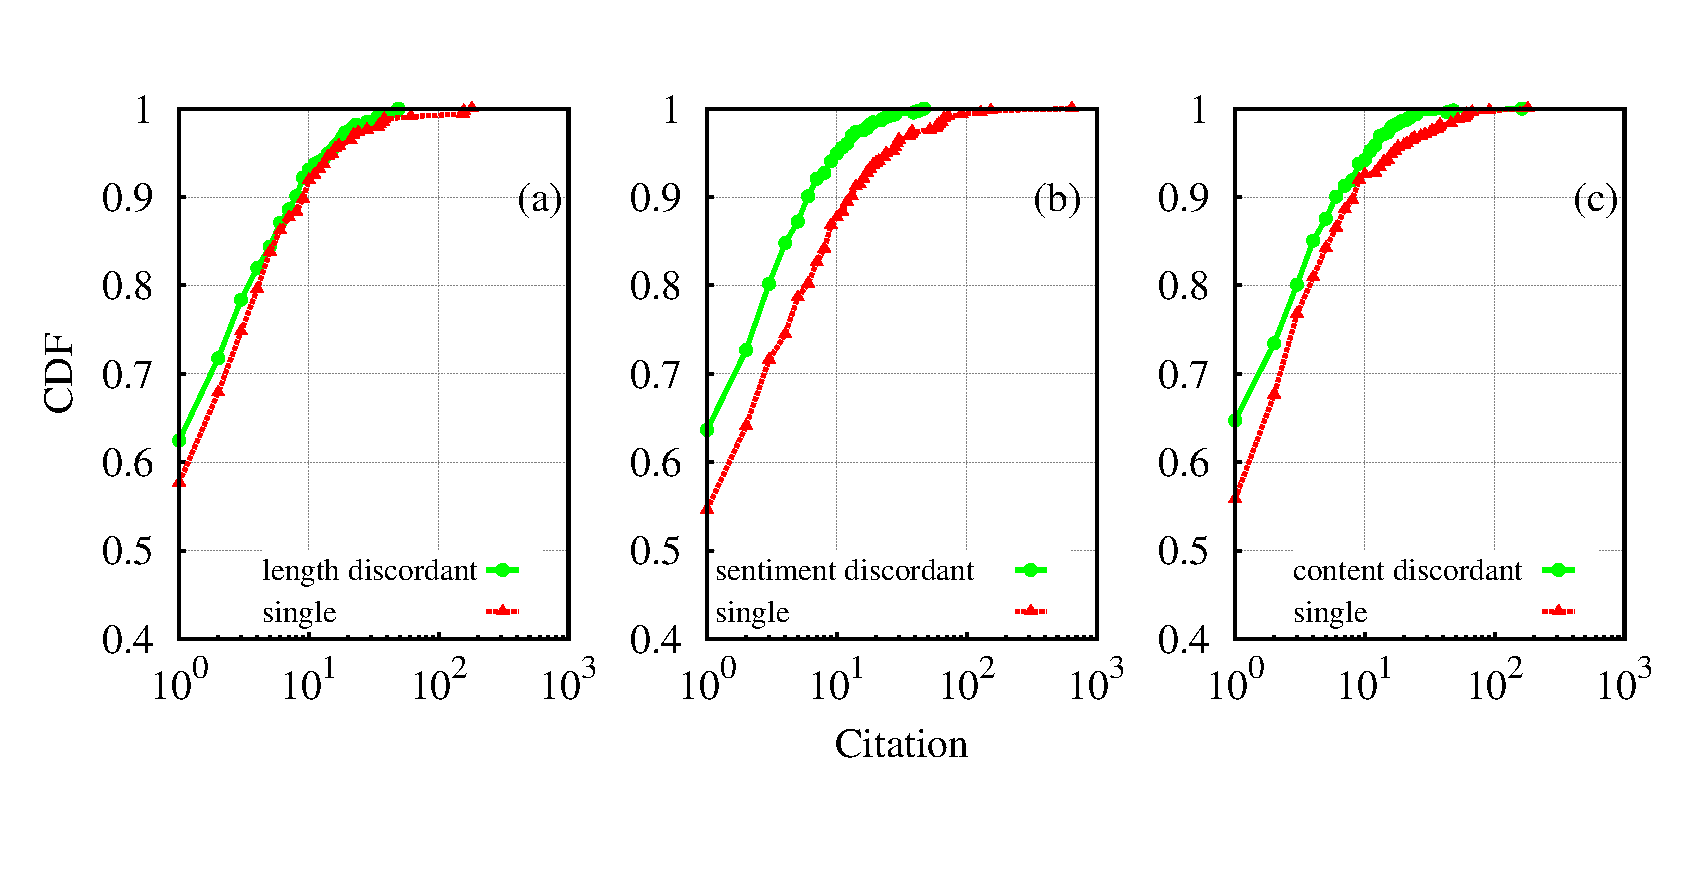
\includegraphics[scale = 0.3]{./texfiles/Chapter_4/cikm_17/figures/citation_mul_all_dis.eps}
 \caption{\label{con:citation_dis} Cumulative distribution function of citations for single refereed papers and discordant multi-refereed papers in terms of (a) length, (b) sentiment 
 and (c) content for JSTAT.} 
 %We randomly selected single-reviewed papers equal in number to the discordant multi-reviewed sets for each type.}
\end{figure}

\medskip


\noindent
\subsection{Analyzing reviewer tendencies}
\label{reviewer}
%\mycheckng{What percentage of reviewers are anomalous}
Reviewers are assigned with the responsibility of judging the quality of a submitted paper and hence their knowledge and training is highly critical. 
In fact, the decision of acceptance or rejection of a paper depends on the reviewer's perception of the paper. 

%\begin{figure}
% \centering
% \includegraphics[scale = 0.26]{figures/reviewer.eps}
% \caption{\label{reviewer} Cumulative distribution function of fraction of cases a reviewer was a part of a multi-referee system across all the reviewers
% for both JHEP and JSTAT datasets.}
%\end{figure}



%We calculate for each reviewer the fraction of cases where he is a part of a multi-referee set among his total assignments and plot the 
%cumulative distribution function of this fraction in figure~\ref{reviewer} for both JHEP and JSTAT datasets. The figure clearly indicates 
%that for JHEP the reviewers are mostly part of a single-referee set up while for JSTAT, the reviewers are part of a multi-referee set up in many more cases. 

% \begin{figure} 
%  \centering
%  \includegraphics[scale = 0.26]{figures/ed_ref_comb.eps}
%  \caption{\label{reviewer} Cumulative distribution function of the fraction of cases a reviewer is a part of a multi-referee system across all the reviewers for JHEP and JSTAT datasets.}\end{figure}
\begin{figure}
 \centering
 \includegraphics[scale = 0.3]{./texfiles/Chapter_4/cikm_17/figures/citation_delay_acpt_ratio_jhep.eps}
 \caption{\label{a_d_jhep} Mean citation versus (a) accept ratio (b) assignment delay buckets for the JHEP dataset. 
 Note that the papers are segregated into accept ratio/delay bins and the mean citation is calculated for each bin. 
 Typical bin sizes for accept ratio are $<0.1$,$(\geq 0.1$ and $<0.2)$ and so on while for delay the sizes are $<100$, $(\geq 100$ and $< 200)$ and so on.\vspace{4mm}}
\vspace{3mm}
 \end{figure}

%We further leverage the technique introduced in~\cite{sikdar2016anomalies} and identify the set of under-performing
% reviewers for both the datasets. 
% \mycheck{put in the definition of underperforming/anomalous-----}
In the last section we defined a referee/editor to be anomalous (under-performing) if - \\
(i) papers accepted by him/her have low citation (research wrongly judged to be impactful)\\
(ii) papers rejected by him/her have high citation (quality research wrongly judged as flawed)\\
%In fact, the authors propose a method for identifying under-performing (anomalous) referees/editors. Leveraging on the same method we observe that  
% the proportion of referees classified as under-performing are approximately $26\%$ and $21\%$ respectively for JHEP and JSTAT datasets.
%The authors hypothesize that accepted papers receiving low citation as well as rejected papers receiving high citations are anomalous cases as 
%ideally they should have been respectively rejected and accepted.  
We make the following general observations - \\
(i) If we consider all the cases where an under-performing editor assigned multiple reviewers for a submission, in $69.8\%$ cases 
at least one of them was under-performing. This indicates that unless the reviewers are selected carefully, chances are it might lead to wrong judgment.\\
(ii) Under-performing reviewers when part of a multi-referee system tend to do a better judgment as compared to cases when they serve as single reviewers.
This is illustrated by the fact that average citation of the accepted  papers reviewed by multiple reviewers with at least one under-performing reviewer ($32.4$) 
is more compared to that of the papers reviewed by a single anomalous reviewer ($18.2$) across the two datasets.
%\vspace{-4mm}
\subsubsection{Factors determining performance of the referees}
We next look into factors that could be used to quantify the performance of the reviewers. The quantification can be used as a 
fitness value for assignment of a new submission (we use these to calculate these quantities in a later section to develop a scheme for automatic referee group selection). 
Given a submission, we identify two factors that are indicative of reviewer fitness (i) accept ratio and (ii) time since the last assignment.\\
\noindent(i) \textit{Accept ratio}: Given a submission, we consider for each reviewer ($i$) the fraction of papers (s)he has accepted at the time of submission. 
We denote this by $a_i$. To show that it is indeed an indicator we consider all the accepted and the rejected papers as well as their assigned reviewers. 
We then calculate the accept ratio of the assigned reviewers and compare them against the citations received by each of them. 
In figures~\ref{a_d_jhep}(a) (JHEP) and~\ref{a_d_jstat}(a) (JSTAT) we plot the accept ratio against the citations received by the accepted as well as the rejected papers. 
Note that we bin the papers based on the accept ratio and calculate the average citation in each case. The typical bin sizes are $\leq 0.1$, $(> 0.1$ and $\leq 0.2)$ and so on. 
We hence obtain $10$ such bins numbered 1-10. 
In case of multi-referee papers the average accept ratio of the reviewers is considered. We observe that for both the datasets very high accept ratio or a very low accept 
ratio might lead to wrong judgment. \\ 
\noindent(ii) \textit{Time since last assignment}: Given a submission and its corresponding submission date we calculate for each reviewer ($i$) the time (in days) between the 
last review assignment date and the submission date (denoted by $d_i$). To illustrate the rationale, we again consider all the accepted and the rejected papers and calculate 
the delay for the assigned reviewers. We again bin the delay values and calculate the average citation (refer to figures~\ref{a_d_jhep}(b) and~\ref{a_d_jstat}(b)). Typical bin 
sizes are $\leq 100$, $(> 100$ and $\leq 200)$ and so on (10 such bins are obtained numbered 1-10). We observe that the reviewers who are assigned very close to their last 
assignment or those who have not been assigned for a long time often fail to correctly judge the quality of the paper correctly as the papers accepted by them are cited less 
on average while those rejected are cited more. 


% \begin{figure}
%  \centering
%  \includegraphics[scale = 0.26]{figures/citation_delay_acpt_ratio_jhep.eps}
%  \caption{\label{a_d_jhep} Mean citation versus (a) accept ratio (b) assignment delay buckets for the JHEP dataset. 
%  Note that the papers are segregated into accept ratio/delay bins and the mean citation is calculated for each bin. 
%  Typical bin sizes for accept ratio are $<0.1$,$(\geq 0.1$ and $<0.2)$ and so on while for delay the sizes are $<100$, $(\geq 100$ and $< 200)$ and so on.}
% \end{figure}

\begin{figure}
 \centering
 \includegraphics[scale = 0.3]{./texfiles/Chapter_4/cikm_17/figures/citation_delay_acpt_ratio_jstat.eps}
 \caption{\label{a_d_jstat} Mean citation versus (a) accept ratio (b) assignment delay buckets for JSTAT dataset. Note that the papers are 
 segregated into accept ratio/delay bins and the mean citation is calculated for each bin. Bin sizes are same as figure \ref{a_d_jhep}.\vspace{4mm}}
\vspace{3mm}
 \end{figure}



\subsubsection{Action with under-performing reviewers}
A naive solution could be to not assign the under-performing reviewers and only assign the best performing ones, but this is not always feasible 
since the number of referees is limited and they often decline assignments. Hence a better solution would be to group them such that the overall performance improves. 
To this aim, we first divide the reviewers into 3 classes separately for accept ratio and time 
since last assignment. A reviewer $i$ with accept ratio $a_i < 0.3$ is assigned ``Low'' (L), with $0.3 \leq a_i < 0.6$ is assigned ``Medium'' (M) and with $a_i \geq 0.6$ is 
assigned ``High'' (H). Note that reviewers in M were the best performing referees (refer to figures \ref{a_d_jhep}(a) and \ref{a_d_jstat}(a)). Each multi-refereed paper 
(by exactly 2 referees) is classified into one of the six classes (LL, MM, HH, LH, MH, LH) based on the class of each referee and the average citation of the papers in each 
class is noted (figure \ref{ref_perf}(a)). We observe that when both the referees belong to the M class (MM) the performance is naturally well. More importantly, reviewers in L and H class 
perform better when paired with a referee from M class (even better than MM). On repeating the same experiment with time since last assignment, 
we observe a similar trend (figure \ref{ref_perf}(b)) with MM class performing the best followed by MH and LM.  
Note that in this case reviewers with $d_i < 100$ are assigned class L, with $100 \leq d_i < 300$ are assigned M and rest are assigned H. 
%This indicates that grouping 
%reviewers while assigning multiple referees for a 
%submission is highly critical toward improving the effectiveness of the system. 
%We further look into the proportion of discordant cases for each reviewer combination. 
More importantly the discordant cases mostly occur for 
class combinations LL, HH and LH (refer to table \ref{tab:dis}). In fact, MM has the least proportion of discordant cases. 
This further indicates the correct reviewer grouping is critical in curtailing the discordant cases which is one of the prime reasons behind the multi-reviewer system failing. 
Note that the above results are obtained for JHEP dataset and a similar pattern is observed 
for JSTAT as well.

\begin{figure}
 \centering
 \includegraphics[scale = 0.3]{./texfiles/Chapter_4/cikm_17/figures/ref_performance.eps}
 \caption{\label{ref_perf} Mean citation for papers belonging particular class combination with respect to (a) accept ratio (b) time since last assignment. For example LL would represent a paper reviewed by referees both 
 belonging to class L.\vspace{4mm}}
\end{figure}







\medskip


\noindent
\subsection{Forming reviewer groups}
\label{group}

The results in the previous section together lead us to believe that the editors in numerous cases fail to assign reviewers which may further lead to flawed papers 
being accepted into the literature while at 
the same time quality research being overlooked. We hence proceed to propose a framework that could recommend compatible referee groups which could then be assigned to 
a submitted paper. 
Note that such a system would be required to - \\
(i) recommend multiple items (referees) to a single user (submission).\\ 
(ii) recommend only homogeneous (compatible) items together while making multiple recommendations. \\ 
(iii) provide a scheme to rank the groups since there could be numerous compatible groups and recommending all of them would be infeasible. \\
Genetic algorithm has already been found to be very effective in obtaining desired groups in collaborative learning setting \cite{moreno2012genetic,ani2010method} 
and we argue that assigning multiple referees to a submission is similar to forming 
compatible referee groups. More importantly, for such a framework a scheme for ranking the groups is inherently present (we provide a detailed description later in this section).   
We hence leverage the idea of GA based team formation framework to obtain the best possible combination of referees which might lead to better judgment of the quality 
of the work. 
%In specific, we use a genetic algorithm framework to obtain the best possible referee assignments for a given paper. Note 
%\mycheck{why GA?}

%hence we leverage this framework to obtain the best possible multiple-referee assignments for a given paper.

\begin{table}
\centering
\caption{Proportion of discordant cases (length, sentiment and content) in each reviewer class combination with respect to (accept ratio, time since 
last assignment).\vspace{3mm} }
\label{tab:dis}
\begin{tabular}{c|c|c|c}
\hline
           & Length       & Sentiment    & Content      \\ \hline
MM         & 0.176, 0.159  & 0.194, 0.143 & 0.164, 0.152 \\ 
LM, HM     & 0.173, 0.162 & 0.243, 0.192 & 0.237, 0.216 \\ 
LL, HH, LH & 0.312, 0.254 & 0.371, 0.286 & 0.293, 0.311 \\ \hline
\end{tabular}
\vspace{4mm}
\end{table}

\subsubsection{Problem definition} Given a submission $S$, a set of reviewers $R = \{R_1, R_2,\ldots, R_n\}$ and the number 
of reviewers to be assigned for a paper $k$, the goal is to obtain a set of potential reviewer groups $G = \{ G_1, G_2, \ldots, G_u\}$ (each of size $k$) 
who could be assigned to referee a submission.

\subsubsection{Methodology}
We now proceed to develop a solution to the above problem based on a genetic algorithm framework which is inspired by the method proposed in~\cite{ani2010method}. 
Typically, chromosomes are represented as simple
strings of data and instruction. In our case chromosomes represent solutions while reviewers are chosen as genes. The details of our algorithm is as follows -- 
\subsubsection*{Selecting a population} Genetic algorithm starts with an initial population represented by the chromosomes. 
Ideally the assigned reviewers should be knowledgeable and experienced in the topics related to the submitted paper. Although information about the associated topic of the papers are not present, each paper in the dataset is  associated with a set of keywords (at least 1 and at most 4, assigned by the publisher) which we use as a proxy for the topic. While the JHEP dataset consists of 201 unique keywords, JSTAT dataset has 562. This again indicates that the papers in JSTAT are more diverse. 
Hence for  a given 
submission we first extract the keywords. 
%As mentioned earlier the keywords are used as a proxy for the topic of the paper. Note that a better way would be to explicitly obtain the topic of the paper, but due to lack of information we use the keywords. In case the topics are explicitly available, it can be easily incorporated into our framework. 
Given the keywords, we extract from the pool of referees only those peers who have reviewed, till the date of the submission in question, at least one paper 
that has one (or more) keywords in common with that of the submission. This set ($\bar R$) represents the potential population of reviewers for the query paper.

% \begin{figure}
%  \centering
%  \includegraphics[scale = 0.26]{figures/topic.eps}
%  \caption{\label{topic} Cumulative distribution function of the fraction of papers being multi-refereed across all the keywords for both JHEP and JSTAT datasets.}
% \end{figure}


\subsubsection*{Initialization} Once the initial population $\bar R$ of reviewers is obtained, we classify them based on 
the accept ratio and time from the last assignment. For each reviewer $i$ we obtain the accept ratio $a_{i}$ and time from the last 
assignment $d_i$ (scaled between 0 and 1). Finally, we calculate the fitness score for the reviewer $i$ as -
\begin{equation}
 f_i = \alpha \ast a_i + (1-\alpha)\ast d_i
\end{equation}
where $\alpha$ is a tuning parameter. Based on the fitness score we classify each reviewer into one of the three classes. Reviewers with fitness score 
less than $0.33$ are classified as class 1 ($RC_1$), between $0.33$ and $0.66$ are classified as class 2 ($RC_2$) and the rest as class 3 ($RC_3$). 
We then club the reviewers randomly into non-overlapping groups of size $k$. This forms the initial generation with each group represented as 
a chromosome. Note that a generation forms a solution set for the above problem.

\subsubsection*{Fitness evaluation}
Once a generation is obtained, we proceed to calculate the fitness of each chromosome (group) and, thereby, calculate the fitness of the whole generation. 
The generation level fitness ($FG_{gen}$) is calculated according to function 1 for a generation $gen$. For each class $RC_i$ we initially calculate the number of reviewers in $RC_i$ 
per group (represented by $RPC_i$). Now for every group $g_j$ we find the number of reviewers of each class $RC_i$  which we represent by $RC_{i}^{g_j}$. We penalize the 
chromosome if the constraint (refer to line 10 of function 1) is violated by not adding anything to the final score; otherwise, a value of 1000 is added to the fitness score.
Note that $1000$ is a representative value and for practical purposes we can use any positive value ($C$). 
More importantly, this scoring scheme further allows for ranking the groups. 
\begin{function1}
 \caption{generation\_level\_fitness()}
 $G$, $RC_i$ \\ 
 $FG_{gen} \leftarrow$ 0\\
 $|G|\leftarrow$ Number of groups\\
 $|RC_i|\leftarrow$ Number of peers in $RC_i$\\
 $|RPC_i|\leftarrow$ Number of peers of class $RC_i$ per group (i.e., $|RPC_i| = |RC_i|/|G|$) \\
 $|RC_{i}^{g_j}|\leftarrow$ Number of actual peers of class $RC_{i}$ in $g_j$\\
 \For{each group $g_j \in G$}{
 \For{each $RC_i$}{
 \If{$|RC_{i}^{g_j}|\geq |RPC_i|$}{
  $FG_{gen} = FG_{gen} + 1000$\\
      } 
    }
 }
 \Return{$FG_{gen}$}
\end{function1}
%\vspace{-8mm}
%\mycheck{An example to illustrate the computation of the above fitness would be nice.Sandipan: added}



To illustrate on how the fitness function is calculated we consider here a toy example. Consider a population of 16 reviewers (with ids 0 - 15), group size of 4 and 3 reviewer classes (1, 2, 3) with number of reviewers in each class being 6, 5 and 5 respectively. Let the reviewers with ids 0 - 5 be assigned to class 1, 6 - 10 to class 2 and rest are assigned to class 3. 
So, $|RPC_1| = 1.5$, $|RPC_2| = 1.25$ and $|RPC_3| = 1.25$.
%\mycheck{The calculation is not correct. Check $|RPC_3| = 1.25$} 
Each generation consists of 4 groups. Let us consider a group $g$ with reviewers 0, 1, 6 and 12. For this group  $|RC_1^{g}| = 2$, $|RC_2^{g}| = 1$ and $|RC_3^{g}| = 1$. Since $|RC_1^{g}| > RPC_1$, it contributes a score of 1000. Similarly, $|RC_2^{g}|$ and $|RC_3^{g}|$ does not contribute to any score. 
%\mycheck{According to your example $|RC_3^{g}| < |RPC_3|$ and therefore should not add a score of 1000. CHECK.} 
Hence the score contributed by this group to the generation is 1000. Sum of this score across all the groups in the generation equals the generation level fitness. 
Note that our algorithm is inherently fair because the proportion of referees in each class is maintained in the recommended set of referees.

\begin{figure}
\centering
\includegraphics[scale=0.32]{./texfiles/Chapter_4/cikm_17/figures/cross_over.pdf}
\caption{\label{c_o} Crossover technique used in our framework}
\vspace{4mm}
\end{figure}

\subsubsection*{Crossover}
Crossover is the process in which two chromosomes combine the genetic material to create a new generation such that the new one possesses the genetic material of both. 
Although several techniques for crossover exist~\cite{golberg1989genetic}, we here consider the one-point crossover technique. 
One random position in the chromosome is chosen to determine the crossover point. In the offsprings produced, the data till the crossover point are copied verbatim from the parents while the data beyond the crossover point are swapped between the two parents. As a result, these new chromosomes or
offsprings share some similar features from the parents chosen. If the crossover is not applied, offsprings are exact copies
of the parents. Crossover technique is illustrated in figure \ref{c_o}.
We have set the crossover rate for our experiments to 70\%. 
Note that mutation process can also be used to maintain genetic diversity but we only stick to crossover for our experiments. 
The process of crossover is repeated several times and the fitness score of the generation is calculated each time. The generation 
with the best score is confirmed as the best possible reviewer grouping for the submitted paper.

\begin{figure}
\centering
\includegraphics[scale=0.32]{./texfiles/Chapter_4/cikm_17/figures/r_d_g.pdf}
\caption{\label{r_d_g} Block diagram demonstrating the work flow of our system.}
\vspace{4mm}
\end{figure}

\subsubsection{Evaluation}

To evaluate the performance of our algorithm, we initially separate out the multi-refereed papers from both the datasets. Based on the long term citations received by each, 
we classify them as high and low cited. Specifically we rank them based on their citations and top 25 percentile are classified as highly cited ones and bottom 25 percentile 
are classified as low cited ones. The classification is done separately across both accepted and rejected papers. We hypothesize that - \\
(i) For accepted papers, highly cited papers represent the cases where the reviewer group was chosen correctly. Moreover, if the reviewer group which was originally assigned 
the paper is also one of the groups recommended by our algorithm, we consider it as a true positive case.\\
(ii) Similarly for rejected papers, low cited papers also represent the cases where the reviewer group was chosen correctly and if our recommendation matches we consider 
it as true positive as well.\\
(iii) For accepted papers, low cited papers represent the cases where the reviewer group was not chosen correctly. If for such a paper the original reviewer group does not feature in the 
list of recommended groups, we consider it as true negative. \\ 
(iv) Similarly, for rejected papers, high cited papers also represent the cases where the reviewer group was not chosen correctly and our hypothesis follows. \\
Since our algorithm allows for ranking of the groups based on the fitness score, we recommend top $k$ (how the results vary with $k$ is shown later) percentile groups. A block diagram representing the work flow of our system is presented in figure \ref{r_d_g}.
%Note that we recommend top $k$ percentile instead of recommending a fixed number as in traditional case. This is because the candidate set of groups is not fixed and grows with 
%time.

% \begin{figure}
% \centering
% \includegraphics[scale=0.32]{./texfiles/Chapter_4/cikm_17/figures/r_d_g.pdf}
% \caption{\label{r_d_g} Block diagram demonstrating the work flow of our system.}
% \end{figure}

%\mycheck{put in the parameter estimation values}
\begin{figure}
\centering
\includegraphics[scale = 0.35]{./texfiles/Chapter_4/cikm_17/figures/param_estimate.eps}
\caption{\label{fig:param_estimte} Mean true positive (averaged over accepted and rejected papers) value while recommending a set of reviewer groups for papers across different values 
of (a) $\alpha$ and (b) crossover rate. Experiments repeated for both JHEP and JSTAT datasets. $k = 15$}
\vspace{4mm}
\end{figure}
%\vspace{2mm}

{\bf Sensitivity to the parameters:}
As mentioned earlier, our algorithm requires two parameters, (i) $\alpha$ and (ii) the crossover rate. In figure~\ref{fig:param_estimte}(a) we plot the true positive rate 
for different values of $\alpha$. We observe that TP (averaged over accepted and rejected cases) improves with increasing value of $\alpha$ after which it drops for 
both JHEP and JSTAT datasets. Optimal result is obtained at $\alpha = 0.6$ for JHEP and $\alpha = 0.7$ for JSTAT. 
We hence set the value of $\alpha$ at 0.6 and 0.7 respectively for JHEP and JSTAT datasets. \\
We further look into the crossover rate as well. In figure~\ref{fig:param_estimte}(b), we plot TP for different crossover rates. 
%TP is observed to be lower for 
%low crossover rate. 
%This is because lower crossover rate allows for very low change of the chromosomes. On the other hand, for very high crossover rate changes in the chromosome occurs at higher rates which increases the chances of obtaining the best solution. 
Optimal TP is obtained at 70\% crossover rate and hence we set the crossover rate at $70\%$ for our experiments. The number of generations we examine is set at 500.\\ 

{\bf Key results:}  
For both JHEP and JSTAT mostly two reviewers are assigned per submission albeit there are cases where three reviewers have also been assigned. 
For generating the results, we only consider the cases where the number of assigned reviewers were two. We calculate for each reviewer the accept ratio and time from the last assignment at the point of submission. 
We then run our algorithm for each submission falling in highly cited and low cited accepted and rejected papers. 
Note that we rank the papers based on citations it has accrued and consider the top and bottom 25 percentile 
to be high and low cited papers respectively. 
%25 percentile category. \mycheck{This is misleading? 25 percentile category of WHAT? Nothing is clear.} 
In table~\ref{tab:k} we present the true positive and true negative values for both JSTAT and JHEP at different values of $k$ (note that we rank the groups based 
on the fitness score and recommend groups in the top $k$ percentile). 
With $k = 15$, for JHEP we could recommend the correct group of reviewers in $81\%$ 
of the cases (represented by the true positive value) for accepted papers and $75\%$ of the cases for rejected papers. Similarly, we could correctly identify $84\%$ of the true negative cases for the accepted papers and $73\%$ for the rejected papers. Corresponding values for JSTAT are 
$79\%$ (accepted), $75\%$ (rejected) and $81\%$ (accepted), $71\%$ (rejected) respectively. %\mycheck{I think you can also report MRR. Can we report NDCG also?} 
These results indicate that our algorithm is indeed very effective in recommending referee pairs. We further look into the cases where 
our algorithm failed to obtain the correct grouping. We observe that in most of these cases a new reviewer (without any previous review history) was assigned. 
Since our algorithm recommends reviewers leveraging the review history, these cases were missed.
%For cases where three reviewers were assigned, our algorithm could correctly recommend at least two referees in 
%$73\%$ cases on average across accepted and rejected papers for JHEP and $69\%$ for JSTAT. 
We further check our results for $k=5$ and $k=10$ which are also reported in 
table~\ref{tab:k}. With $k=5$ we were able to obtain TP of 0.61 and 0.59 respectively for accepted and rejected papers in case of JHEP. For JSTAT the corresponding values 
are 0.63 and 0.59. More importantly we could obtain a high TN of 0.91 (accepted) and 0.89 (rejected) for JHEP and 0.92, 0.82 for JSTAT. This is because we are 
recommending a smaller number of groups which reduces the possibility of recommending a particular undesired/desired group.



{\bf Comparison with baseline algorithms:}
As our algorithm presents computational overhead a natural question to ask is whether it is worth it. We hence design a simple 
baseline (random) to compete with our algorithm. For a submission, initial population of suitable reviewers is obtained (in the same way as our GA based algorithm) and each reviewer is classified into one of L, M, H categories. A subset of reviewers is then selected randomly in such a way that the proportion of reviewers in each class (in the population) is maintained 
in the chosen set. 
We then randomly form groups of types MM, ML and MH since these are the best performing reviewer groups (refer to figure \ref{ref_perf}).  
To compare, we obtain the same number of groups as obtained from our proposed algorithm. 
%hence we check if the originally assigned group of reviewers is present 
%in the recommended set (which is considerably larger than our recommended set since all random pairings of referees are part of this set). 
We further consider two other 
ablation type baselines - (i) GA with only accept ratio (only $a_i$, fitness score is calculated with only $a_i$), (ii) GA with only time since last assignment 
(only $d_i$, fitness score calculated with only $d_i$). Note that this can be achieved by setting $\alpha$ to 1 and 0 respectively. 
In figure~\ref{fig:GA_base} we plot the TP and TN for 
the baseline algorithms and our proposed algorithm ($k$ is set at 15). 
We consider five random instances and report the mean value for the baseline. We observe TP (averaged over accepted and rejected cases) 
to be much lower (0.37 (JHEP) and 0.45 (JSTAT) for random, 0.51 and 0.53 for only $a_i$, 0.42 and 0.37 for only $d_i$) compared to our algorithm. 
 TN is compared to be higher because of the less possibility of randomly obtaining a particular undesired/desired group.  
As a second level of evaluation we further consider overlap in the set of groups proposed by our 
algorithm with those obtained from the baseline algorithm. The purpose of this is to show that the top $k$ groups proposed by our algorithm based on the fitness function cannot be obtained 
through random allocation. In specific, we measure the Jaccard similarity between the set of groups obtained through baseline and those obtained through our algorithm. Across 
all the papers we obtain a low similarity value of 0.31 which further corroborates our hypothesis.\\
%\mycheck{Two other ablation type baselines could be: Our GA framework with the fitness score calculated base on (i) only accept ratio and (ii) time since last assignment.}

%\begin{figure}
%\includegraphics[scale = 0.26]{figures/G_A_all.eps}
%\caption{\label{fig:G_A} True positive (TP) and true negative (TN) cases while recommending a set of reviewer groups for both accepted and rejected papers for (a) JHEP and (b) JSTAT datsets.}
%\end{figure}

\begin{table}[]
\centering
\caption{True positive (TP) and true negative (TN) values across accepted and rejected papers measured for different values of $k$. Results are reported for JHEP and JSTAT datasets.}
\label{tab:k}
%\resizebox{!}{1.5cm}{
\begin{tabular}{c|c c|c c}
\hline
        & \multicolumn{2}{c|}{JHEP}                                                                                                   & \multicolumn{2}{c}{JSTAT}                                                                                                  \\ \hline
K       & \begin{tabular}[c]{@{}c@{}}TP\\ (accept,reject)\end{tabular} & \begin{tabular}[c]{@{}c@{}}TN\\ (accept,reject)\end{tabular} & \begin{tabular}[c]{@{}c@{}}TP\\ (accept,reject)\end{tabular} & \begin{tabular}[c]{@{}c@{}}TN\\ (accept,reject)\end{tabular} \\ \hline
5       &  0.61,0.59                                                   &  0.91,0.87                                                   &   0.63,0.59                                                  & 0.92,0.82                                                             \\ 
10      &  0.72,0.66                                                   &  0.87,0.79                                                   &   0.73,0.71                                                  & 0.85,0.76                                                             \\ 
15      &  0.81,0.75                                                   &  0.84,0.73                                                   &   0.79,0.74                                                  & 0.81,0.71                                                             \\ \hline \hline
Average &  0.71,0.66                                                   &  0.87,0.80                                                   &   0.72,0.68                                                  & 0.86,0.76                                                             \\ \hline
\end{tabular}%}
\vspace{5mm}
\end{table}



\if{0}
\mycheck{Discard this part?}
\noindent{\bf{Further refinements:}} We observed in the previous section that under-performing reviewers when clubbed together often send in contradicting review reports. More specifically, 
reviewer class combinations of HH and LL contributes to a major proportion of discordant cases. We leverage this result and remove all the groups of class 
combinations HH and LL from the recommended set of reviewer groups. We observe that the size of the recommended set reduces on an average by 22.75\% for 
JHEP and around 22\% for JSTAT dataset (refer to figure \ref{fig:G_A_mod}). For JHEP dataset TP cases reduces to $76\%$ from $81\%$ for accepted and to $71.3\%$ 
from $75\%$ for rejected papers while the TN case improves to $86\%$ and $81\%$ for accepted and rejected papers respectively. The corresponding values for 
JSTAT dataset are $76\%$ ($79\%$), $71\%$ ($75\%$), $83\%$ ($81\%$) and $74\%$ ($71\%$). Hence with only very marginal change in accuracy we are able to recommend 
an even smaller set of reviewer groups. 

\begin{figure}
\includegraphics[scale = 0.26]{figures/G_A_all_mod.eps}
\caption{\label{fig:G_A_mod} True positive (TP) and true negative (TN) cases while recommending a set of reviewer groups for both accepted and rejected papers 
for (a) JHEP and (b) JSTAT after removing HH and LL reviewer class combinations. $k = 15$}
\end{figure}
\fi

\medskip

\vspace{-6mm}
\noindent
\section{Importance of the editor}
\label{editor_imp}

Results from the previous section suggests that given the reviewer history and the related topic, our algorithm is able to correctly recommend a set of reviewers. It might therefore be tempting to believe that a peer-review system can be made to function without even the intervention of the editor. However, we would like to point out that this is not the case and our system simply recommends a set of reviewer groups to the editor from which (s)he has to use his/her expertise and knowledge to choose the most appropriate group. In fact the intervention of the editor to select the reviewer group for each paper is critical to the performance of our scheme in the long run. To illustrate this, we perform the following experiment. The multi-refereed papers are sorted based on their date of submission. The reviewer history for each referee is included till the point of submission of the first multi-refereed paper. For each paper our system recommends a set of reviewer groups; if we consider no editor intervention in our system, the top ranked (according to fitness score) reviewer group is selected from the set of recommended groups and the 
reviewer history updated accordingly. Note that for our original system, we assumed the editor selected the correct set of reviewers and the reviewer history was updated following the original assignment. Also since, in this simulation settings, we do not know whether the reviewers would have actually accepted or rejected the paper, we flag the paper as accepted with a probability proportional to the current average accept ratio of the assigned referees. The system is allowed to evolve following the above mentioned way.   

\begin{figure}
\centering
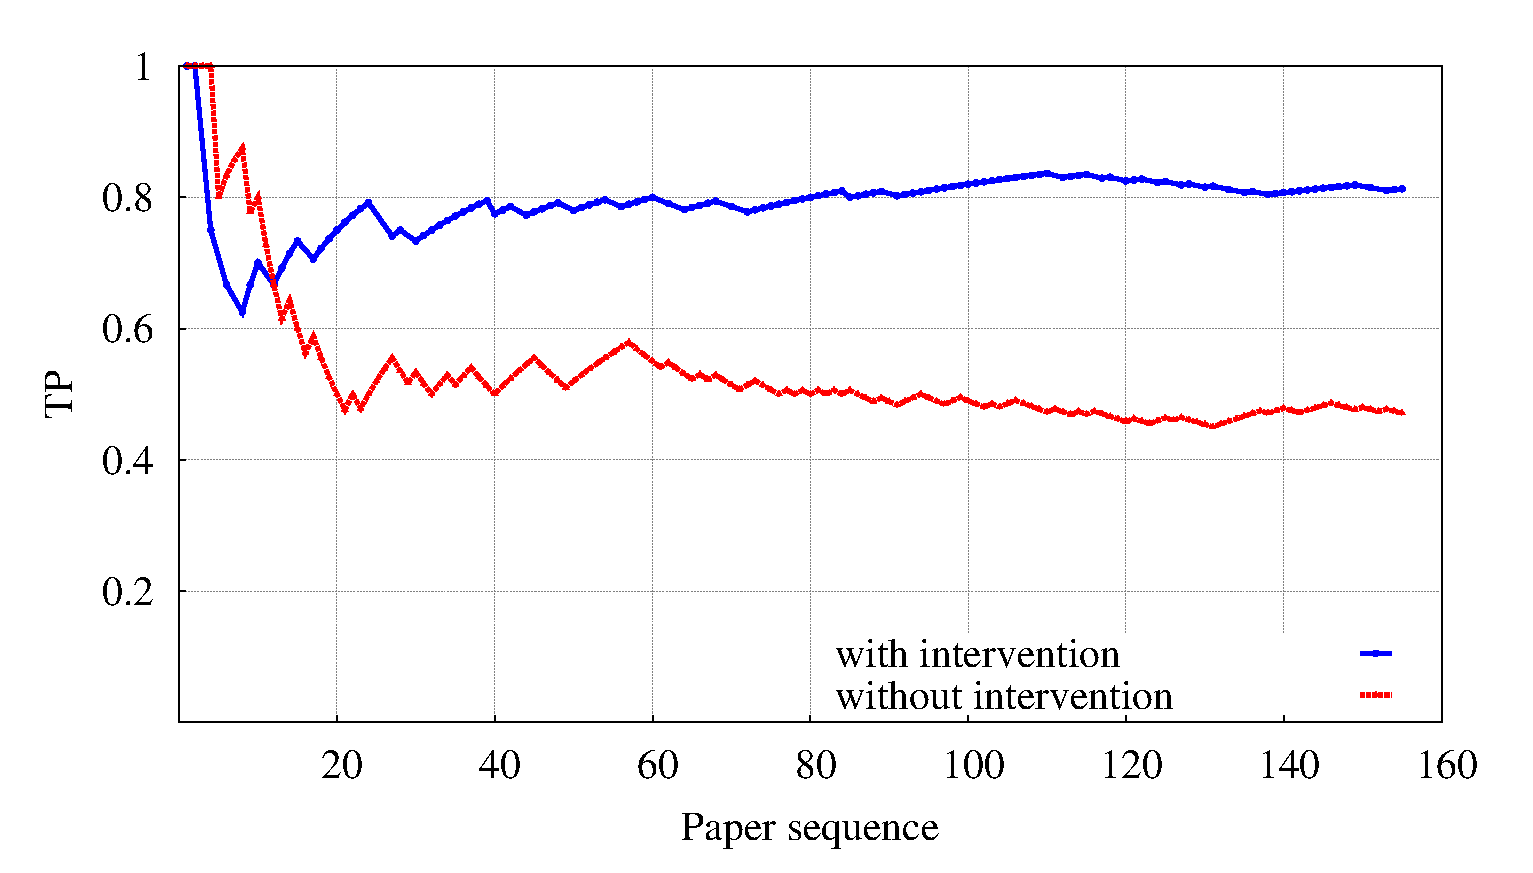
\includegraphics[scale = 0.26]{./texfiles/Chapter_4/cikm_17/figures/G_A_comp.eps}
\caption{\label{fig:ed_imp}True positive value at each point of recommendation of the top 25 percentile (based on citation) accepted papers for JHEP dataset. 
The papers are sorted by date of submission and x-axis denotes the paper number in the sequence.}
\vspace{4mm}
\end{figure}
\medskip

We now consider the top 25 percentile papers (based on citation) and sort them according to the date of submission. The simulation setup above is then used to recommend a set of reviewer groups. In figure~\ref{fig:ed_imp} we plot the TP value for each paper sorted according to their submission dates. Specifically, we calculate the fraction of correct recommendations at the point of every new submission for both the original system (with editor intervention) and the simulation system (without intervention). We observe that the performance of the system without intervention degrades alarmingly over time compared to the original system. The above results indicate that the expert intervention of the editor in choosing the reviewer groups is extremely important toward proper functioning of the peer-review system. 



